\documentclass[10pt,a4paper]{article}
\usepackage[margin=0.6in]{geometry}
\usepackage{enumitem}
\usepackage{booktabs}
\usepackage{graphicx}
\usepackage{hyperref}
\usepackage{titlesec}
\usepackage{parskip}
\usepackage{multicol}
\usepackage{caption}

% Section spacing
\titlespacing*{\section}{0pt}{15pt}{6pt}
\titlespacing*{\subsection}{0pt}{6pt}{3pt}
\titleformat{\section}{\normalfont\normalsize\bfseries}{\thesection.}{0.4em}{}
\titleformat{\subsection}{\normalfont\small\bfseries}{\thesubsection}{0.4em}{}
\setlength{\parskip}{5.5pt}
\setlength{\parindent}{0pt}

\pagestyle{plain}

\begin{document}

\begin{center}
{\Large \textbf{SceneIQ: Phase 1 Progress Report}} \\[3pt]
{\normalsize MSML640 -- Computer Vision, Spring 2026}
\end{center}

\vspace{2pt}

\textbf{Group Number:} 12 \hfill \textbf{Team Name:} SceneIQ

\vspace{2pt}
\begin{center}
\begin{tabular}{cll}
\toprule
\textbf{Member} & \textbf{Name} & \textbf{UID} \\
\midrule
1 & Siddhi Rohan Chakka & 121302823 \\
2 & Krishna Kishore Buddi & 121142672 \\
3 & Dhanush Vasa & 121227645 \\
\bottomrule
\end{tabular}
\end{center}

\section{Revised Problem Statement}

Object detection and segmentation have gotten very good, but most vision systems never ask whether a scene actually makes sense. A penguin sitting in a kitchen or a boat in a desert would not raise any flags for a standard detector. SceneIQ is our attempt to close that gap: given a single RGB photograph, classify it as coherent or incoherent. We built a benchmark from Visual Genome scene graphs and synthetic copy-paste augmentation, and we solve the task by fine-tuning a Vision Transformer.

\section{Progress Since Proposal}

Our original proposal had three goals: (1) binary coherence classification with F1 $\geq$75\%, (2) localization of inconsistent elements via per-patch heatmaps, and (3) an ablation comparing ViT-only, GAT-only, and a fused model.

Since then, we finished the data pipeline (downloading VG, mining co-occurrences, generating synthetic incoherent images, assembling train/val/test splits), trained a ViT-base classifier for 10 epochs on 15,000 images, and evaluated on the held-out test set. The classification system is functional and already clears our F1 target. We estimate the project is about 80\% done.

The main change from the proposal is that we split the work into two phases. Phase 1 gets the ViT-only classifier working as a baseline. Phase 2 adds scene-graph fusion (GAT + cross-attention) and localization heatmaps. We went this route because trying to build and debug everything at once made it hard to tell what was actually helping. Getting a clean baseline first means the ablation study will produce more useful comparisons.

For training, we fine-tuned \texttt{google/vit-base-patch16-224} (ImageNet-21k pretrained) with a 2-class head, AdamW optimizer (lr = $2 \times 10^{-5}$), batch size 32, for 10 epochs. Best checkpoint was selected by validation accuracy. We ran training locally on an NVIDIA RTX 3060 GPU.

Test results against our proposal targets:

\vspace{2pt}
\begin{minipage}[t]{0.48\textwidth}
\centering
\small
\begin{tabular}{@{}lcc@{}}
\toprule
\textbf{Metric} & \textbf{Test} & \textbf{Target} \\
\midrule
Accuracy & 94.4\% & -- \\
Precision & 92.0\% & -- \\
Recall & 90.9\% & -- \\
F1 & 91.5\% & $\geq$75\% \\
ROC-AUC & 97.8\% & -- \\
\bottomrule
\end{tabular}
\end{minipage}
\hfill
\begin{minipage}[t]{0.48\textwidth}
\centering
\small
\begin{tabular}{@{}lcc@{}}
\toprule
\textbf{Epoch} & \textbf{Val Acc} & \textbf{Val F1} \\
\midrule
1 & 94.2\% & 0.910 \\
2 & 95.1\% & 0.924 \\
6 (best) & 95.2\% & 0.927 \\
10 (final) & 94.9\% & 0.923 \\
\bottomrule
\end{tabular}
\end{minipage}

\vspace{4pt}

\begin{minipage}[t]{0.48\textwidth}
\centering
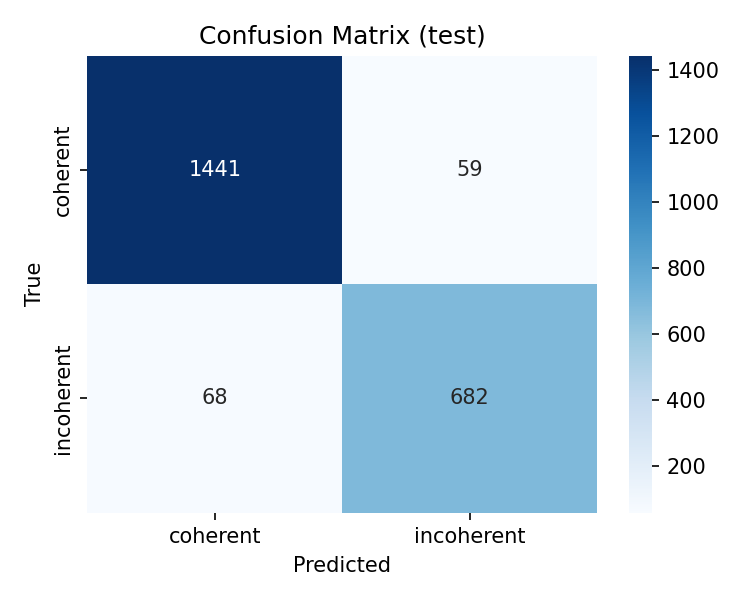
\includegraphics[width=1.08\textwidth]{confusion_matrix.png}
\captionof{figure}{Confusion matrix on test split (n=2250).}
\end{minipage}
\hfill
\begin{minipage}[t]{0.48\textwidth}
\centering
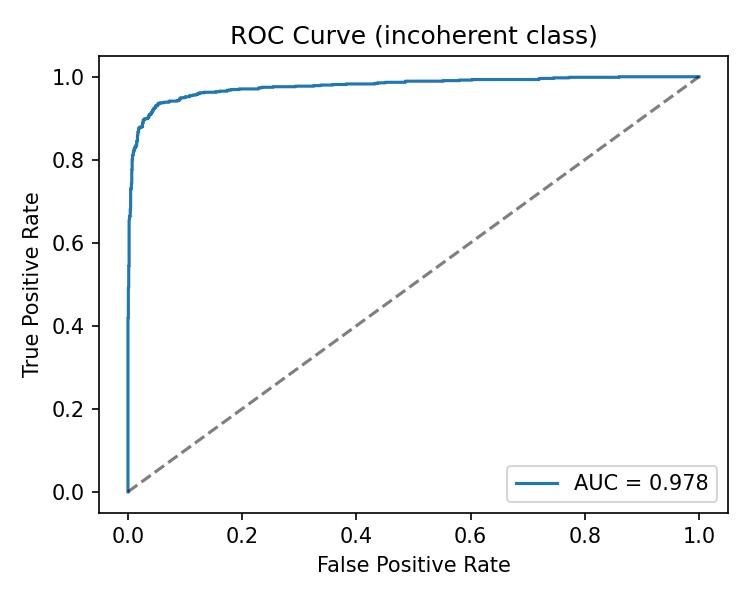
\includegraphics[width=1.08\textwidth]{roc_curve.png}
\captionof{figure}{ROC curve (AUC=0.978).}
\end{minipage}

\vspace{4pt}

The test split has 1,500 coherent and 750 incoherent images, all held out during training. Coherent images are real VG photographs with varying scenes, lighting, and quality. The model got 1,441 of 1,500 coherent images right and 682 of 750 incoherent ones. When we broke down incoherent performance by alien object type, abstract categories like ``patterns'' and ``instructions'' had the lowest recall (33\%), while concrete objects like furniture and vehicles were above 90\%.

Midway through development we added two quality filters to the synthetic generation pipeline (minimum alien frequency and minimum crop size) which removed a lot of bad training samples and helped convergence. The trained checkpoint (\texttt{models/best.pt}) and the evaluation pipeline both work end-to-end; running \texttt{evaluate.py} on a new test split produces all metrics and plots automatically.

\section{Team Integration Status}

Rohan wrote the data pipeline scripts and training code. Krishna worked on co-occurrence analysis and the synthetic augmentation logic. Dhanush handled the evaluation metrics and visualization scripts. Everything is version-controlled on GitHub.

\section{Challenges and Solutions}

\begin{enumerate}[itemsep=10pt,leftmargin=1.5em]
    \item \textbf{Bad synthetic samples.} The first runs of \texttt{generate\_synthetic.py} produced a lot of garbage. Alien object crops would shrink to a few pixels after resizing, or the pasted object would be invisible against the background. Out of 10,372 attempts, we were throwing away more than half. We fixed this with two filters: \texttt{--min-alien-count 50} drops alien categories with fewer than 50 VG instances (these tend to be noisy or mislabelled), and \texttt{--min-crop-size 32} rejects any crop smaller than 32$\times$32 px. After adding both, the acceptance rate is 48\% (5,000/10,372) and every accepted image has a clearly visible alien object.

    \item \textbf{Leakage between splits.} We caught a subtle issue: VG images that were used as destination scenes during copy-paste could also appear in the coherent split. If the model memorized those backgrounds, it would get a free shortcut instead of learning about object coherence. We fixed this in \texttt{prepare\_dataset.py} by tracking the 5,000 scene IDs used during synthesis and removing them from the coherent pool before splitting (108,077 $\to$ 103,077 eligible images).

    \item \textbf{Overfitting past epoch 6.} Training accuracy hit 100\% by epoch 5, but validation accuracy sat around 95\% and validation loss kept going up (0.15 at epoch 2 to 0.30 by epoch 10). We use best-checkpoint selection, so the final saved model is from epoch 6 (val acc = 95.2\%) and the overfit later epochs are discarded. For Phase 2 we plan to add augmentation (random crops, color jitter) and dropout to see if we can push validation higher.
\end{enumerate}

\section{Next Steps for Final Phase}

\begin{enumerate}[itemsep=10pt,leftmargin=1.5em]
    \item Build the scene-graph fusion module: a GAT encoder over RelTR-extracted scene graphs, fused with ViT patch features via cross-attention (as described in the proposal).
    \item Run the ablation study comparing ViT-only (91.5\% F1), GAT-only, and the full fusion model to see if scene-graph structure actually adds anything on top of raw visual features.
    \item Add per-patch inconsistency scoring for localization heatmaps. Evaluate pointing accuracy against ground-truth alien bounding boxes (target $\geq$45\%).
    \item Try regularization strategies (Albumentations augmentation, dropout, early stopping) to address the overfitting we saw after epoch 6.
    \item Package the final model as a standalone inference script: image in, Scene Coherence Score out, optional heatmap overlay.
\end{enumerate}

\end{document}
